%
% File acl2021.tex
%
%% Based on the style files for EMNLP 2020, which were
%% Based on the style files for ACL 2020, which were
%% Based on the style files for ACL 2018, NAACL 2018/19, which were
%% Based on the style files for ACL-2015, with some improvements
%%  taken from the NAACL-2016 style
%% Based on the style files for ACL-2014, which were, in turn,
%% based on ACL-2013, ACL-2012, ACL-2011, ACL-2010, ACL-IJCNLP-2009,
%% EACL-2009, IJCNLP-2008...
%% Based on the style files for EACL 2006 by 
%%e.agirre@ehu.es or Sergi.Balari@uab.es
%% and that of ACL 08 by Joakim Nivre and Noah Smith

\documentclass[11pt,a4paper]{article}
\usepackage[hyperref]{acl2021}
\usepackage{times}
\usepackage{makecell}
\usepackage{amsmath}
\usepackage{latexsym}
\usepackage{graphicx} %% inserted
\renewcommand{\UrlFont}{\ttfamily\small}

% This is not strictly necessary, and may be commented out,
% but it will improve the layout of the manuscript,
% and will typically save some space.
\usepackage{microtype}

%\usepackage{fancyhdr} 
%\fancyhf{}
%\cfoot{\thepage}
%\pagestyle{fancy} % page numbering

\aclfinalcopy
%\def\aclpaperid{***} %  Enter the acl Paper ID here

%\setlength\titlebox{5cm}
% You can expand the titlebox if you need extra space
% to show all the authors. Please do not make the titlebox
% smaller than 5cm (the original size); we will check this
% in the camera-ready version and ask you to change it back.

% Content lightly modified from original work by Jesse Dodge and Noah Smith


\newcommand\BibTeX{B\textsc{ib}\TeX}

\title{Reproducibility Project for CS598 DL4H in Spring 2023}

\author{Yu-Chung Lee and Hyeonjae Cho \\
  \texttt{\{ycl7, hc53\}@illinois.edu}
  \\[2em]
  Group ID: 30\\
  Paper ID: 6\\
  Presentation link: \url{https://youtu.be/qMEwlSeE_vk} \\
  Code link: \url{https://github.com/lycpaul/dl4h-gp30-gct}
  } 

\begin{document}
\maketitle

% All sections are mandatory.
% Keep in mind that your page limit is 8, excluding references.
% For specific grading rubrics, please see the project instruction.

\section{Introduction}
\subsection{Citation}
The paper \citep{DBLP:conf/aaai/ChoiXLDFXD20}, published by Google DeepMind, demonstrates that the graph convolutional transformer can handle incomplete or zero structure information of Electronic Health Records data.

\subsection{General Problem}
EHR data have been shown to have an underlying graphical structure that helps improve the performance of the prediction task. However, the previous models treated EHR data in an unordered feature set, disregarding the relationships between diagnoses and treatments. MiME \citep{DBLP:conf/nips/ChoiXSS18} proposed a model that learns the structural information of the EHR data but is still insufficient because many publicly accessible datasets do not provide the reasoning to establish graphic connections, such as claim data. To utilize the hidden hierarchical structure, a more generalized method is needed.

\subsection{The Approach}
The author proposed a GCT network to learn the unknown hierarchical structure of the EHR data by using the self-attention mechanism to obtain a model that allows better classification or prediction performance compared to other baselines that do not consider the hidden graphical structure \citep{DBLP:conf/nips/VaswaniSPUJGKP17}. In addition, they used prior knowledge as an attention mask. We already know that some treatments are necessary for certain diseases, and others are unavailable. Additionally, we can calculate the conditional probabilities among diagnoses, treatments, and laboratory tests based on examples of encounter records. The prior information, illustrated in Figure~\ref{fig:gct-p}, replaces the first GCT block attention layer, which is generally uniformly distributed. As the model goes through further depth blocks, it penalizes if the attention value of the i-th block is quite different from the one of 1st block. Therefore, attention values can imply both a realistic and a novel relationship between nodes.

\begin{figure}
    \centering
    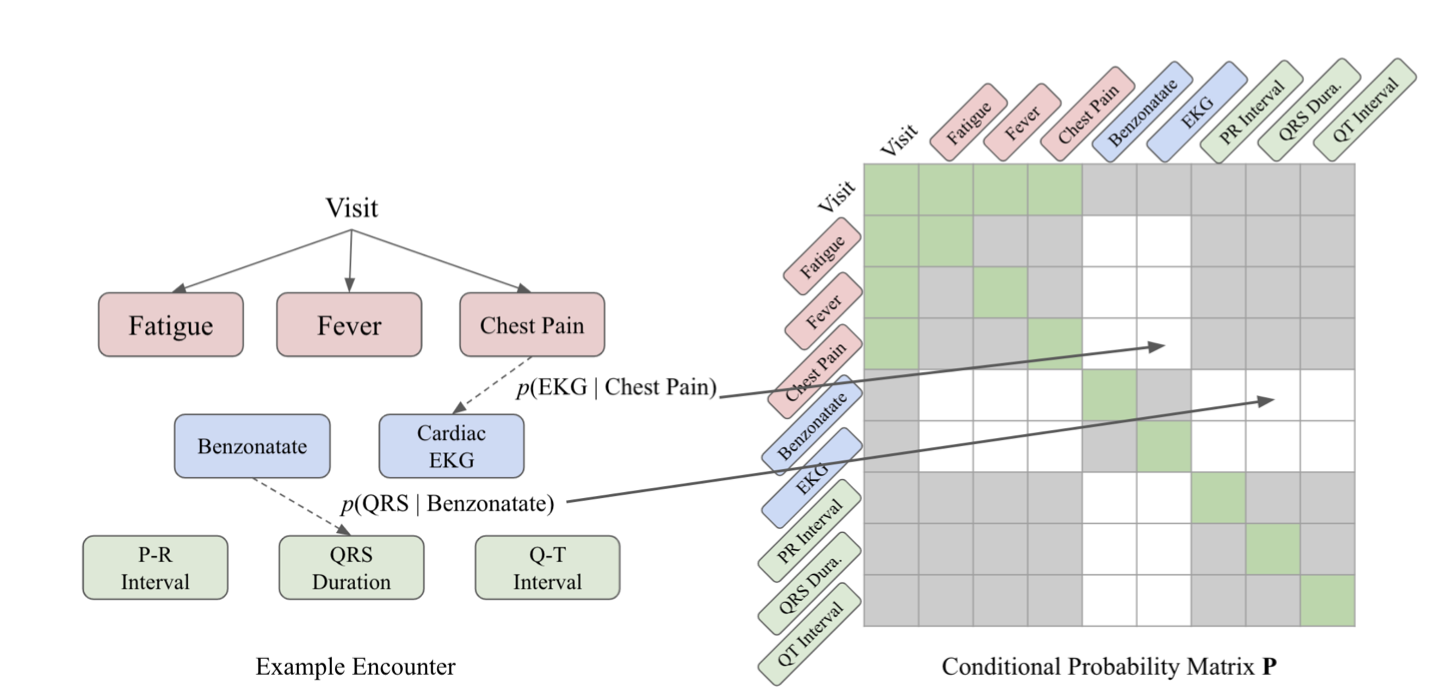
\includegraphics[width=0.45\textwidth]{GCT conditional probability matrix.png}
    \caption{The grey areas indicate not-allowed connections. The green cells show special connections. Conditional probabilities are assigned in corresponding white cells. \citep{DBLP:conf/aaai/ChoiXLDFXD20}}
    \label{fig:gct-p}
\end{figure}

\section{Scope of reproducibility}
The author claims that the GCT model is superior for prediction tasks in a single encounter. Among several experiments conducted in the paper, we plan to reproduce the readmission and mortality prediction task in the eICU dataset and compare it to GCN, which the original paper proposes as benchmarking downstream prediction tasks. We chose the eICU dataset over the synthetic encounter record because the eICU dataset represents real-world EHR data and is considered a close representation of the realistic distribution of diagnostic codes. Therefore, we will verify the claim written in the sub-section below.

We will also evaluate two more baseline models for the prediction tasks: GCN\textsubscript{p}, which is the graph convolution network directly trained based on the conditional probability of preprocessed features, and Transformer, which is the original Transformer implementation with conditional probability as a prior guide, guided mask, and regularization.

\subsection{Addressed claims from the original paper}
In the required downstream prediction task, GCN\textsubscript{p} can utilize the conditional probability as a graph connection to assist the prediction, but such interpretation is noisy and inaccurate. While Transformer can learn the hidden connection, it may struggle to converge without prior guidance. Given that GCT is proposed to train the hidden reasoning connection between diagnostic codes, treatment, and laboratory results with prior knowledge as an initial guide, GCT should combine the strength of GCN\textsubscript{p} and Transformer to deliver a better result. Therefore, two imperial results should be observed:

\begin{itemize}
    \item The graph-convolutional transformer will have AUROC/AUCPR higher than a GCN\textsubscript{p} and Transformer on readmission prediction.
    \item The graph-convolutional transformer will have AUROC/AUCPR higher than a GCN\textsubscript{p} and Transformer on mortality prediction.
\end{itemize}

\section{Methodology}
We first adopted some of the author's code, publicly available on the Google Health GitHub repository\footnote{https://github.com/Google-Health/records-research/tree/master/graph-convolutional-transformer}. We made some minor modifications to make the code compatible with the latest versions of Python 3 and TensorFlow 2, which offer a more stable environment. We also referenced another PyTorch reimplementation of the GCT model \footnote{https://github.com/dchang56/gct-pytorch} and implemented the preprocessing and training pipeline with the PyHealth framework \citep{pyhealth2022github}. The baseline training can be done quickly with the processing pipeline and PyHealth pre-defined models. Descriptive notebooks examples describe the complete training to the evaluation process.

\subsection{Model descriptions}
The proposed model, Graph Convolutional Transformer, combines the concept from the Transformer \citep{DBLP:conf/nips/VaswaniSPUJGKP17} and Graph Convolutional Networks \citep{DBLP:journals/corr/KipfW16}, as the name implies. Especially the Transformer referred to here is an encoder with single-head attention. In addition, GCT does not involve positional embeddings since features in a single encounter are not ordered.

Graph Convolutional Networks (GCN) formulation with known structure information \textbf{A}
\begin{gather*}
    \textbf{C}^{(j)} = \text{MLP}^{(j)}\left(\tilde{\textbf{D}}^{-1} \tilde{\textbf{A}} \textbf{C}^{(j-1)}\textbf{W}^{(j)} \right)
    % \\
    % \textbf{C}^{(j)} = \text{MLP}^{(j)}(\text{softmax} (\frac{\textbf{Q}^{(j)}\textbf{K}^{(j)T}}{\sqrt{d}}) \textbf{C}^{(j-1)}\textbf{W}_\textit{V}^{(j)} )
\end{gather*}

The intuition of the model construction is that: since the actual graph connections are unknown, instead of training the model with the normalized adjacency matrix $\tilde{\textbf{D}}^{-1}\tilde{\textbf{A}}$, we replaced that with the attention map softmax($\frac{\textbf{Q}^{(j)}\textbf{K}^{(j)T}}{\sqrt{d}})$ to learn the underlying connections. In addition, the GCT possesses two known graphical characteristics: First, it uses a mask in the attention generation procedure, which gives negative infinities if the graph connection is not allowed. Second, the regularization formula's loss function restricts the model from inventing unrealistic graph connections. It helps the model discover an underlying graph structure of EHR data in a realistic search space. A simplified model architecture is given in Figure~\ref{fig:gct-a}. Moreover, the learning objective is given below:
\begin{align*}
    \text{Define } \hat{\mathbf{A}}^{(j)} := \text{softmax} (\frac{\textbf{Q}^{(j)}\textbf{K}^{(j)T}}{\sqrt{d}} + \textbf{M} ) \\
    \text{ where } \textbf{Q}^{(j)} = \textbf{C}^{(j-1)}\textbf{W}_\textit{Q}^{(j)}, \\
    \textbf{K}^{(j)} = \textbf{C}^{(j-1)}\textbf{W}_\textit{K}^{(j)}, \\
    \text{d = column size of } \textbf{W}_\textit{K}^{(j)}
\end{align*}
Self-attention:
\begin{gather*}
    \textbf{C}^{(j)} = \text{MLP}^{(j)}\left(\textbf{P}\textbf{C}^{(j-1)}\textbf{W}_\textit{V}^{(j)} \right) \text{ when } j = 1, \\
    \textbf{C}^{(j)} = \text{MLP}^{(j)}\left(\hat{\mathbf{A}}^{(j)}\textbf{C}^{(j-1)}\textbf{W}_\textit{V}^{(j)}\right) \text{ when } j > 1 
\end{gather*}
Regularization:
\begin{gather*}
    \textit{L}_\text{reg}^{(j)} = \textit{D}_\textit{KL} \textbf{(P}\vert\vert\hat{\mathbf{A}}^{(j)}\text{)} \text{ when } j = 1, \\
    \textit{L}_\text{reg}^{(j)} = \textit{D}_\textit{KL} (\hat{\mathbf{A}}^{(j-1)}\vert\vert\hat{\mathbf{A}}^{(j)}) \text{ when } j > 1 \\
    \textit{L} = \textit{L}_\textit{pred} + \lambda\sum_{j}\text{L}_\textit{reg}^{(j)}
\end{gather*}

The above formula contains the observation of the \textit{j}-th convolution layer in a model. \textbf{A} is an adjacency matrix for EHR data, which is an unknown or incomplete structure of an encounter. \textbf{Q} and \textbf{K} represent Query and Value, respectively, which are common vector notations by the attention mechanism. In the self-attention formula, \textbf{C} represents a node embedding, and \textbf{V} stands for a visit. MLP is a multi-layer perceptron located between convolution layers and has its own trainable parameters. \textbf{W} is the trainable parameter of the \textit{j}-th convolution layer. Additionally, GCT proposes two unique techniques, a mask (\textbf{M}) and conditional probabilities (\textbf{P}).

\begin{figure}
    \centering
    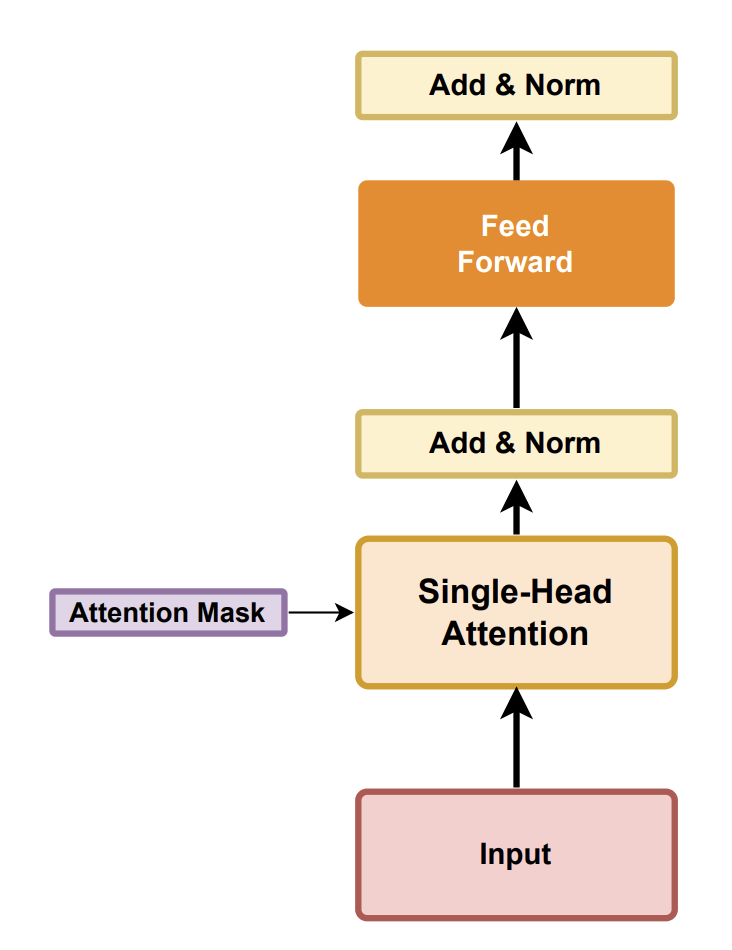
\includegraphics[width=0.25\textwidth]{GCT Architecture.png}
    \caption{Architecture of Graph Convolutional Transformer.}
    \label{fig:gct-a}
\end{figure}


\subsection{Data descriptions}
The eICU dataset includes publicly available\footnote{https://eicu-crd.mit.edu/gettingstarted/access/} de-identified EHR data of over 200,000 ICU admissions from more than 200 hospitals across the United States \citep{DBLP:conf/bcb/JohnsonPCM17},. The dataset contains clinical data such as laboratory results, treatments, diagnoses, and demographic information about the patient, such as age, sex, and ethnicity. To download the dataset, the CITI training program is required.

The eICU dataset contains single encounters that may span over several days. However, the GCT model does not consider time variance, so we only considered a single encounter per patient. The preprocess.py script includes only encounters of less than 24 hours and eliminates duplicated medical codes, such as medications administered multiple times. Moreover, it excludes lab results since they are subject to change over time in the ICU.

The basic statistics of the processed data that were actually used in the model training are as follows:
\begin{table}[h]
    \centering
    \begin{tabular}{c c}
        \Xhline{2\arrayrulewidth}
         & eICU \\
        \hline
        \# of encounters & 41,026 \\
        \# of diagnosis codes & 3,093 \\
        \# of treatment codes & 2,132 \\
        \hline
        Avg. \# of diagnosis per visit & 7.70 \\
        Avg. \# of treatment per visit & 5.03 \\
        \Xhline{2\arrayrulewidth}
    \end{tabular}
    \caption{Statistics of eICU Dataset}
\end{table}

\subsection{Hyperparameters}
We compiled all information regarding hyperparameter settings into a Table  \ref{tab:table}. In addition to the hyperparameters setting provided by the original paper, we also tried different model configurations. We adjusted the parameters to experiment with particular settings' potential effects and improvements, which will be further discussed in the results section.

\begin{table}[h]
\centering
\begin{tabular}{c c c c}
\hline
 & Readmission & Mortality \\
\hline
Batch size & 32 & 32 \\
\hline
MLP dropout rate & 0.08 &  0.72\\
\hline
Post-MLP dropout rate & 0.024 &  0.005\\
\hline
Learning rate & 0.00022 & 0.00011 \\
\hline
Regularization coef. & 0.1 &  1.5\\
\hline
Embedding dim. & 128 & 128 \\
\hline
\# of Transformer stacks & 3 & 3 \\
\hline
\# of attention heads & 1 & 1 \\
\end{tabular}
\caption{Training Hyperparameters for Readmission and Mortality Prediction on eICU as recommended in the original paper.}
\label{tab:table}
\end{table} 

\subsection{Implementation}
The modified Tensorflow 2.0 version of the original source code is available in \footnote{https://github.com/lycpaul/dl4h-gp30-gct/tree/main/gct-tf2} and the modified PyTorch implementation referenced from another open source implementation is available here \footnote{https://github.com/lycpaul/dl4h-gp30-gct/tree/main/gct-pytorch}. Additionally, we also integrate the PyHealth package, creating a new PyTorch training code in \footnote{https://github.com/lycpaul/dl4h-gp30-gct/tree/main/gct-pyhealth}. Furthermore, we have included auxiliary functions, such as attention visualization codes. However, this section will primarily focus on the detailed process of re-implementing and integrating the PyTorch version code into PyHealth. Please refer to Section \ref{subsec:subsectionVisualize} for visualization results.

The PyHealth modules provide a five-stage pipeline modality for all healthcare tasks: loading dataset, prediction tasks labeling, building model, training model, and model inference. By utilizing the datasets parser, and the pipeline design, we have minic a similar training procedure to train our GCT model. We have submitted the changes required to parse the additional tables in eICU datasets to PyHealth (refer to  section \ref{subsec:PyHealthContrib} for details) such that it also allows us to utilize the provided PyHealth AI models as baseline training. All models were trained with Adammax \citet{DBLP:journals/corr/KingmaB14} as the optimizer with linear scheduler instead of the Adam as proposed in the original paper to improve the performance.

\subsection{Computational requirements}
According to the original paper \citep{DBLP:conf/aaai/ChoiXLDFXD20}, both the GCT and the baseline used a system with an Nvidia Tesla P100 with a maximum of 16GB of VRAM. Alternatively, our group reproduced the result with an Nvidia RTX 3090Ti GPU 24GB VRAM system capable of performing the training under the same hyperparameters and settings. In our experiments, GCT implemented with TensorFlow2 will occupy 24GB of VRAM and takes around 8 hours to finish training 1M iterations. Meanwhile, another reimplementation of the GCT model using PyTorch requires less than 3GB VRAM with about 3 hours of training for 1,000,000 iterations.


\section{Results}
% Start with a high-level overview of your results. Does your work support the claims you listed in section 2.1? Keep this section as factual and precise as possible, reserve your judgement and discussion points for the next ``Discussion'' section.

% Go into each individual result you have, say how it relates to one of the claims, and explain what your result is. Logically group related results into sections. Clearly state if you have gone beyond the original paper to run additional experiments and how they relate to the original claims. 

% Tips 1: Be specific and use precise language, e.g. ``we reproduced the accuracy to within 1\% of reported value, that upholds the paper's conclusion that it performs much better than baselines.'' Getting exactly the same number is in most cases infeasible, so you'll need to use your judgement call to decide if your results support the original claim of the paper. 

% Tips 2: You may want to use tables and figures to demonstrate your results.
% % The number of subsections for results should be the same as the number of hypotheses you are trying to verify.

% Results - for the draft, results can be any valuable results. For example, results from a simple baseline model in the paper, from intermediate steps prior to the ultimate target task, or from a tiny subset of the dataset. All those followed by your own analysis can be used. Even if your current results are not as good as the ones in the paper, there must be analyses about what possible reasons and solutions/plans are 
% for Final, All claims should be supported by experiment results
%Discuss with respect to the hypothesis and results from the original paper
%Experiments beyond the original paper
%Credits for each experiment depend on how hard it is to run the experiments. Each experiment should include results and discussion
%Ablation Study.
We have trained the GCT with eICU data on readmission and mortality prediction using the hyperparameters provided by the original paper and several other learning rate and dropout rate setting to see the prediction performance. We have also evaluated Transformer and GCN as the baseline model for mortality prediction.

\subsection{Results}
According to our preliminary result, we noticed that the AUCPR/AUCROC of both predictions of our trained model performed worse than the ones in the paper, even with the hyperparameters stated in the paper. Specifically, the prediction performance is shown in Table \ref{tab:pred_result_table}.

We have already trained the Transformer and GCN against the mortality tasks, and the performance is worse than that of GCT. We also noticed that changing the hyperparameters, such as learning rate, dropout rate, and batch size, would increase the performance.

\begin{table}[htbp]
  \centering
  \caption{Tensorboard plot of our training experiment over the GCT model. The original files and results of other hyperparameters can be viewed in our public repository.}
  \label{tab:tensorboard_table}
  \begin{tabular}{c c}
    \begin{minipage}{0.45\linewidth}
      \centering
      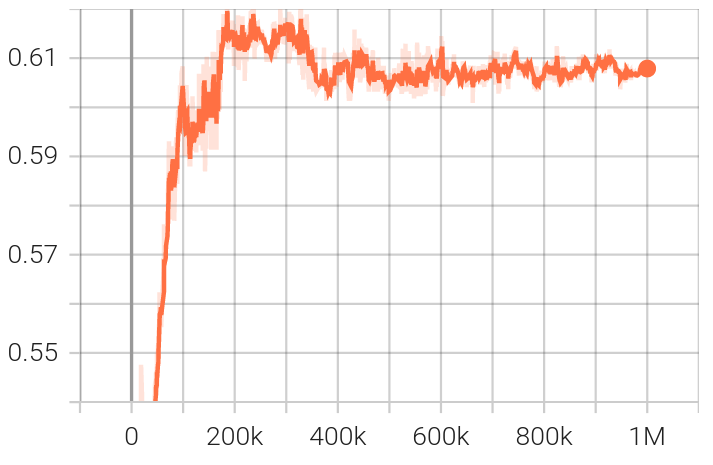
\includegraphics[width=\linewidth]{mortality_eval_aucpr.png}
      \captionsetup{font=footnotesize}
        \caption{AUCPR of mortality prediction.}
    \end{minipage} &
    \begin{minipage}{0.45\linewidth}
      \centering
      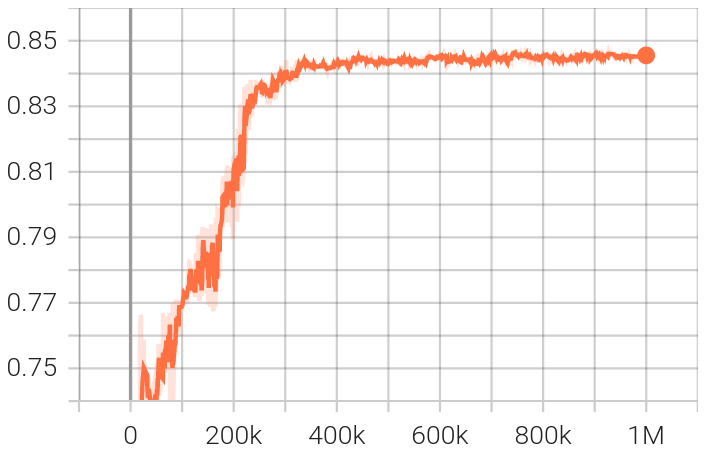
\includegraphics[width=\linewidth]{mortality_eval_auroc.png}
     \captionsetup{font=footnotesize}
        \caption{AUROC of mortality prediction.}
    \end{minipage} \\
    \begin{minipage}{0.45\linewidth}
      \centering
      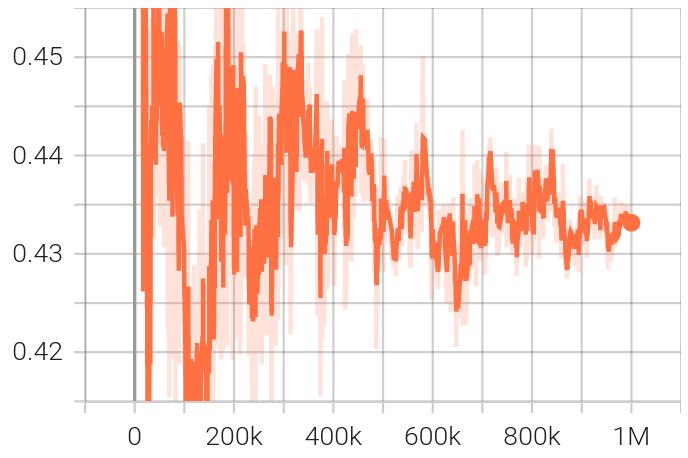
\includegraphics[width=\linewidth]{readmission_eval_aucpr.png}
        \captionsetup{font=footnotesize}
        \caption{AUCPR of readmission prediction.}
    \end{minipage} &
    \begin{minipage}{0.45\linewidth}
      \centering
      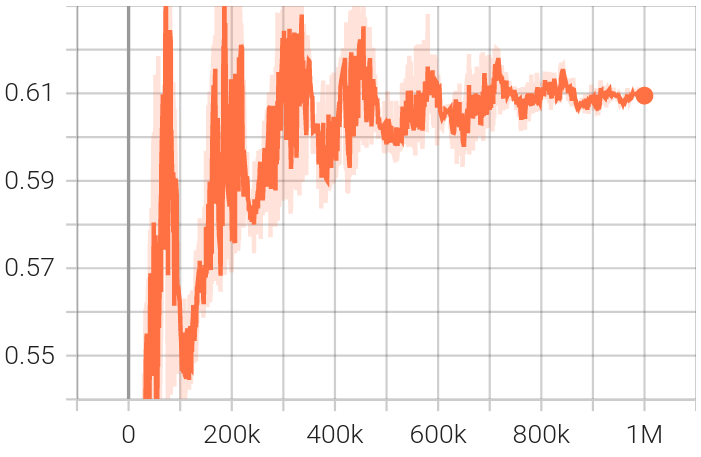
\includegraphics[width=\linewidth]{readmission_eval_auroc.png}
        \captionsetup{font=footnotesize}
        \caption{AUROC of readmission prediction.}
    \end{minipage} \\
  \end{tabular}
\end{table}

\begin{table*}[hbtp]
    \centering
    \begin{tabular}{c c c c c }
        \Xhline{2\arrayrulewidth}
        Tasks & Validation AUCPR & Test AUCPR & Validation AUROC & Test AUROC \\
        \hline
        Readmission (Ours-GCT) & 0.4329 & 0.4081 & 0.6094 & 0.6088 \\
        \hline
        Readmission (Paper-GCT) & 0.5313 & 0.5244 & 0.7525 & 0.7502 \\
        \hline
        Mortality (Ours-GCT) & 0.6079 & 0.5931 & 0.8455 & 0.8118 \\
        \hline
        Mortality (Paper-GCT) & 0.6196 & 0.5992 & 0.9089 & 0.9120 \\
        \hline
        Mortality (Ours-Transformer) & 0.6105 & 0.5585 & 0.8360 & 0.7847 \\
        \hline
        Mortality (Ours-GCN) & 0.4487 & 0.4523 & 0.6735 & 0.6612 \\
        \Xhline{2\arrayrulewidth}
    \end{tabular}
    \caption{Readmission and mortality prediction tasks performance on eICU dataset.}
    \label{tab:pred_result_table}
\end{table*}

\subsection{Additional results not present in the original paper}
\label{subsec:subsectionVisualize}
% Describe any additional experiments beyond the original paper. This could include experimenting with additional datasets, exploring different methods, running more ablations, or tuning the hyperparameters. For each additional experiment, clearly describe which experiment you conducted, its result, and discussions (e.g. what is the indication of the result).
We first evaluate the choice of optimizer and scheduler for the training. We tested with Adam as proposed by the original paper and Adammax, which is a variant of Adam based on the infinity norm. Table \ref{tab:tableExp} shows the improvements in choosing the Adammax with the linear scheduler. Therefore all of our remaining training experiments are conducted with it.

We investigated different post-MLP dropout rates in the output feedforward layer. In this experiment, we freeze other hyperparameters and choose only to evaluate the mortality prediction task. In table \ref{tab:tableExp}, we observed the higher dropout improved the prediction slightly. We also evaluate the effect of stacking self-attention blocks and the usage of multi-head attention. Table \ref{tab:tableExp} indicates that 3 self-attention blocks did improve the performance, which also aligned with the original paper observations that the graphical connections improved and converged better in the third attention block. The multi-head attention also helps improve prediction accuracy.

\begin{table}[h]
\centering
\begin{tabular}{c c c c}
\Xhline{2\arrayrulewidth}
(a) Optimizer, Scheduler & Validation & Test \\
\& learning rate & AUCPR & AUCPR \\
\hline
Adam, none, 1.1e-4 & 0.5340 & 0.5312 \\
\hline
Adammax, linear, 1.1e-4 & 0.5658 & \textbf{0.5974} \\
\hline
Adammax, linear, 1e-3 & \textbf{0.5803} & 0.5844 \\
\Xhline{2\arrayrulewidth}
(b) Post-MLP & Validation & Test \\
dropout rate & AUCPR & AUCPR \\
\hline
0.005 & 0.5658 & 0.5974 \\
\hline
0.2 & 0.5624 & 0.6042 \\
\hline
0.5 & 0.5655 & \textbf{0.6061} \\
\hline
0.72 & \textbf{0.5662} & 0.5971 \\
\Xhline{2\arrayrulewidth}
(c) \# of Attention blocks & Validation & Test \\
\& attention heads & AUCPR & AUCPR \\
\hline
2 blocks 1 heads & 0.5624 & 0.5842 \\
\hline
2 blocks 2 heads & 0.5601 & 0.6102\\
\hline
3 blocks 1 heads & 0.5604 & 0.6042\\
\hline
3 blocks 2 heads & \textbf{0.5759} & \textbf{0.6191}\\
\Xhline{2\arrayrulewidth}
\end{tabular}
\caption{(a) Training results of different optimizers, scheduler, and learning rate combination in mortality prediction. (b) Training results of different post-MLP dropout rates in mortality prediction. (c) Training results of different multi-head and number of Transformer stacks combination in mortality prediction. The learning rate is fixed at 1.1e-4 with post-MLP dropout rate at 0.2.}
\label{tab:tableExp}
\end{table} 

We have implemented a visualization function that facilitates the comprehension of the attention behavior of the transformer block. According to the paper, GCT utilizes prior information power to predict the patient’s outcome better. Therefore, we need to investigate attention maps further to confirm the accuracy of the claim. We have produced a heatmap and a network graph displaying the visit label, actual diagnoses, and treatments. During the processing procedure, the diagnoses and treatment data are concatenated with one visit tensor, resulting in a tensor with a shape of \texttt{(batch\_size, 2*max\_num\_codes+1)}. For compact visualization, we have dropped the padded diagnoses and treatments. Specifically, the heatmap demonstrates which diagnoses led the patient to visit and what treatments were administered. The graph network exhibits thicker edges when the attention value is higher. One can easily understand the relationship between components through the graph network at a glance. For a more detailed interpretation of the graphs, please refer to Figure \ref{fig:attention-map} and \ref{fig:attention-map2}.

\begin{figure}
    \centering
    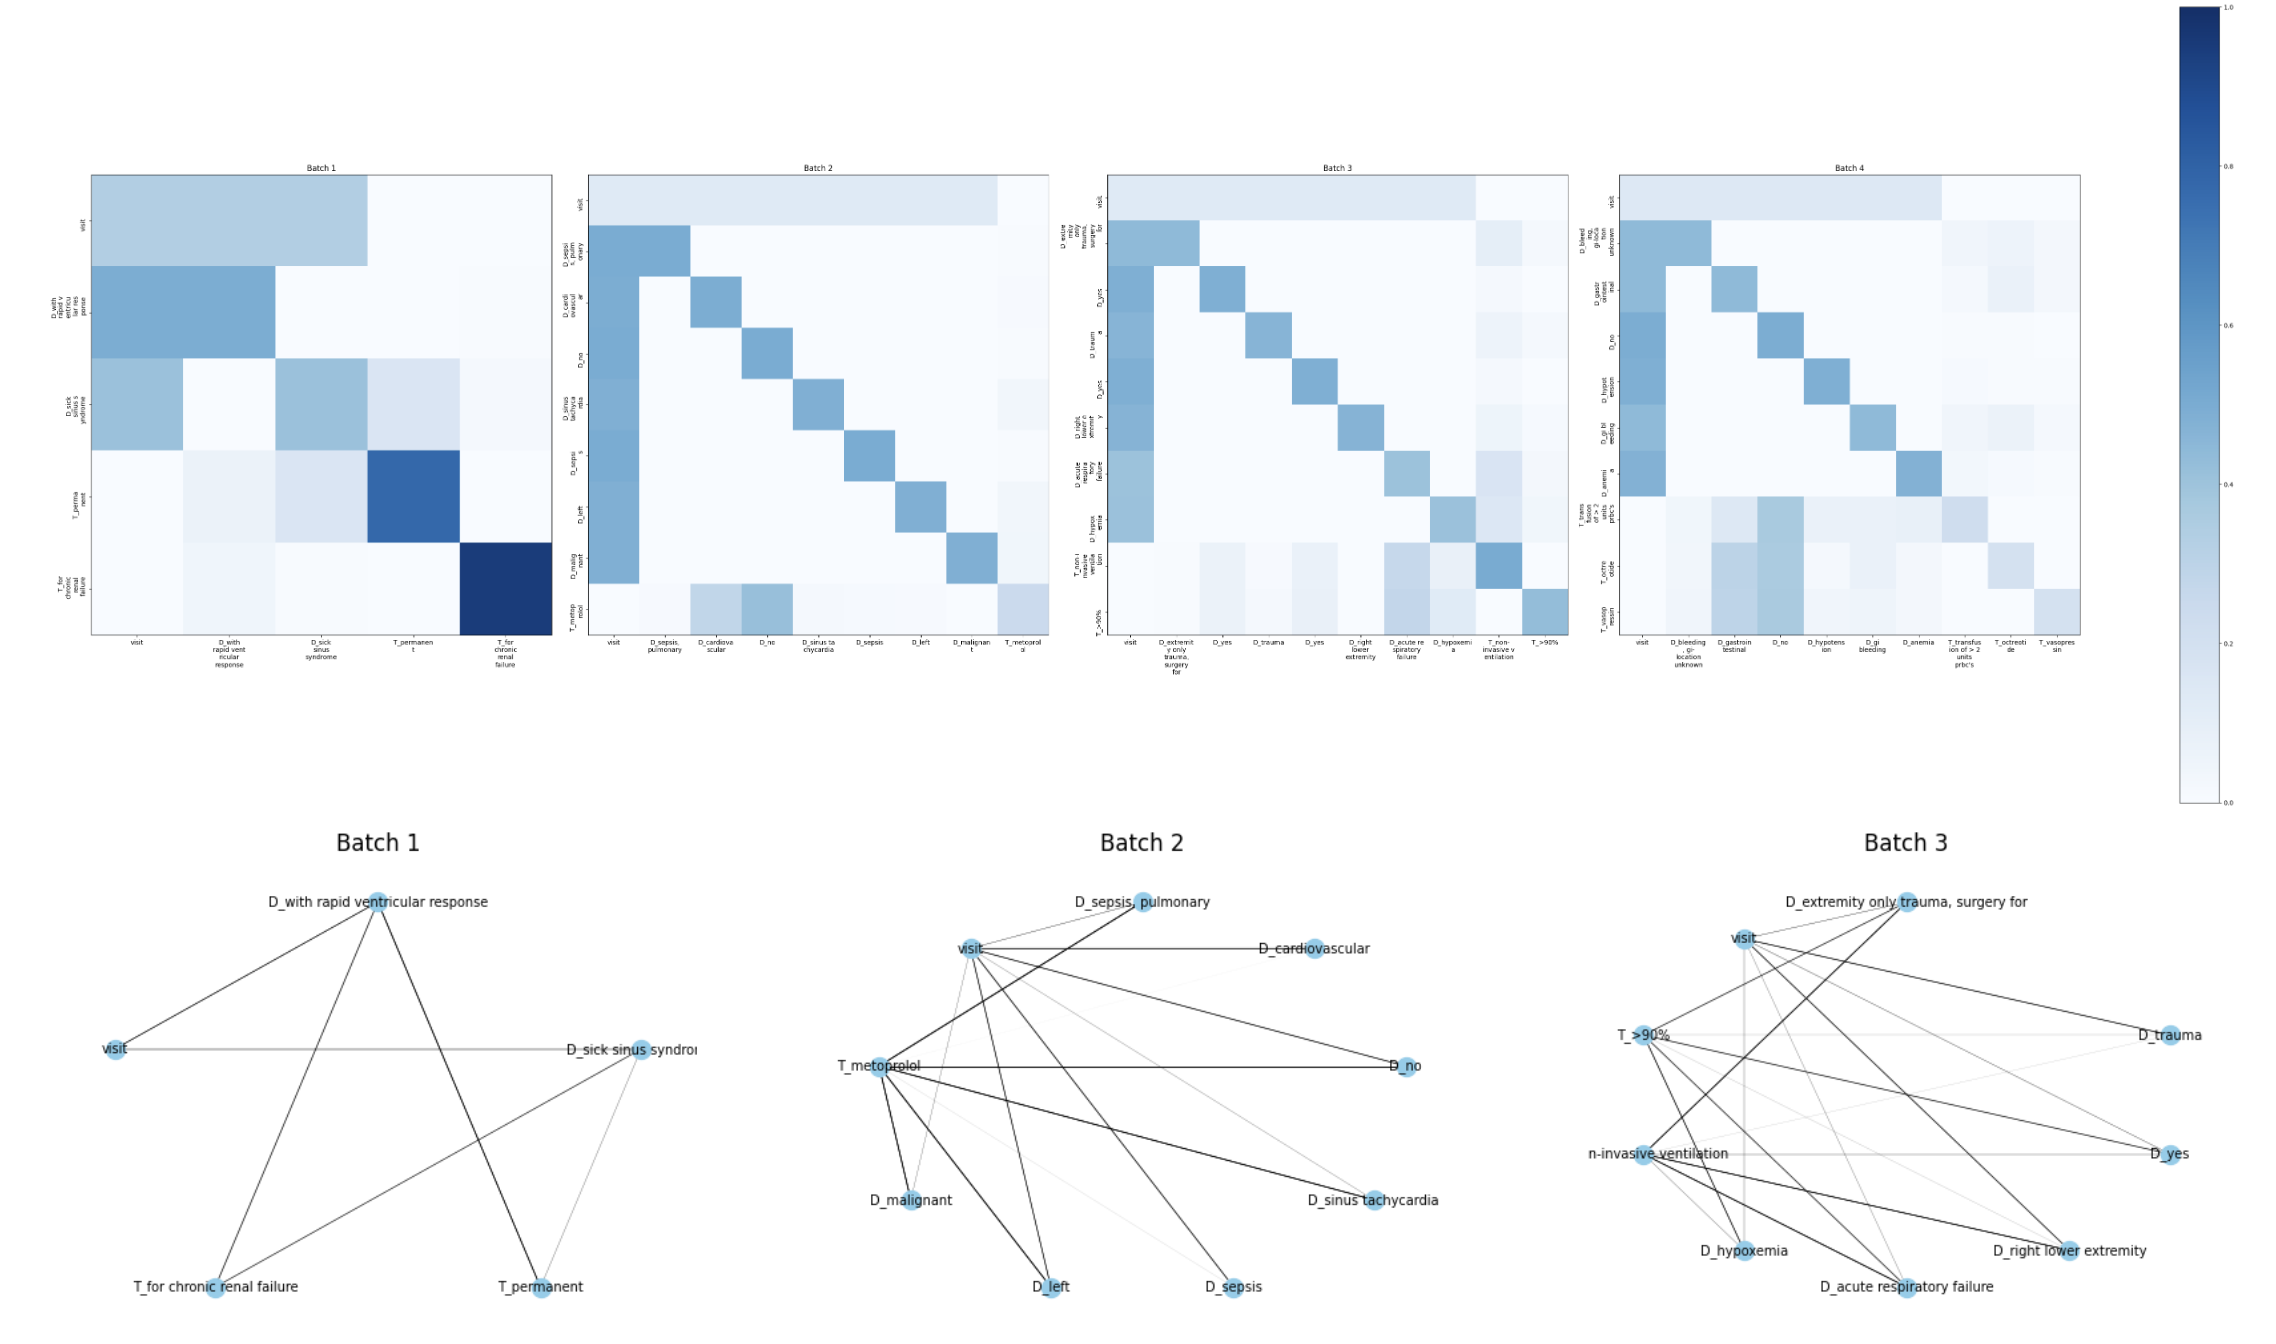
\includegraphics[width=0.5\textwidth]{Attention Map.png}
    \caption{Visualization results in the GCT transformer block. Treatments and diagnoses are denoted with the prefixes `T' and `D', respectively. The full name of each component could not be displayed due to the length limit. (Note: This chart was plotted in one of the early training batches)}
    \label{fig:attention-map}
\end{figure}

\begin{figure}
    \centering
    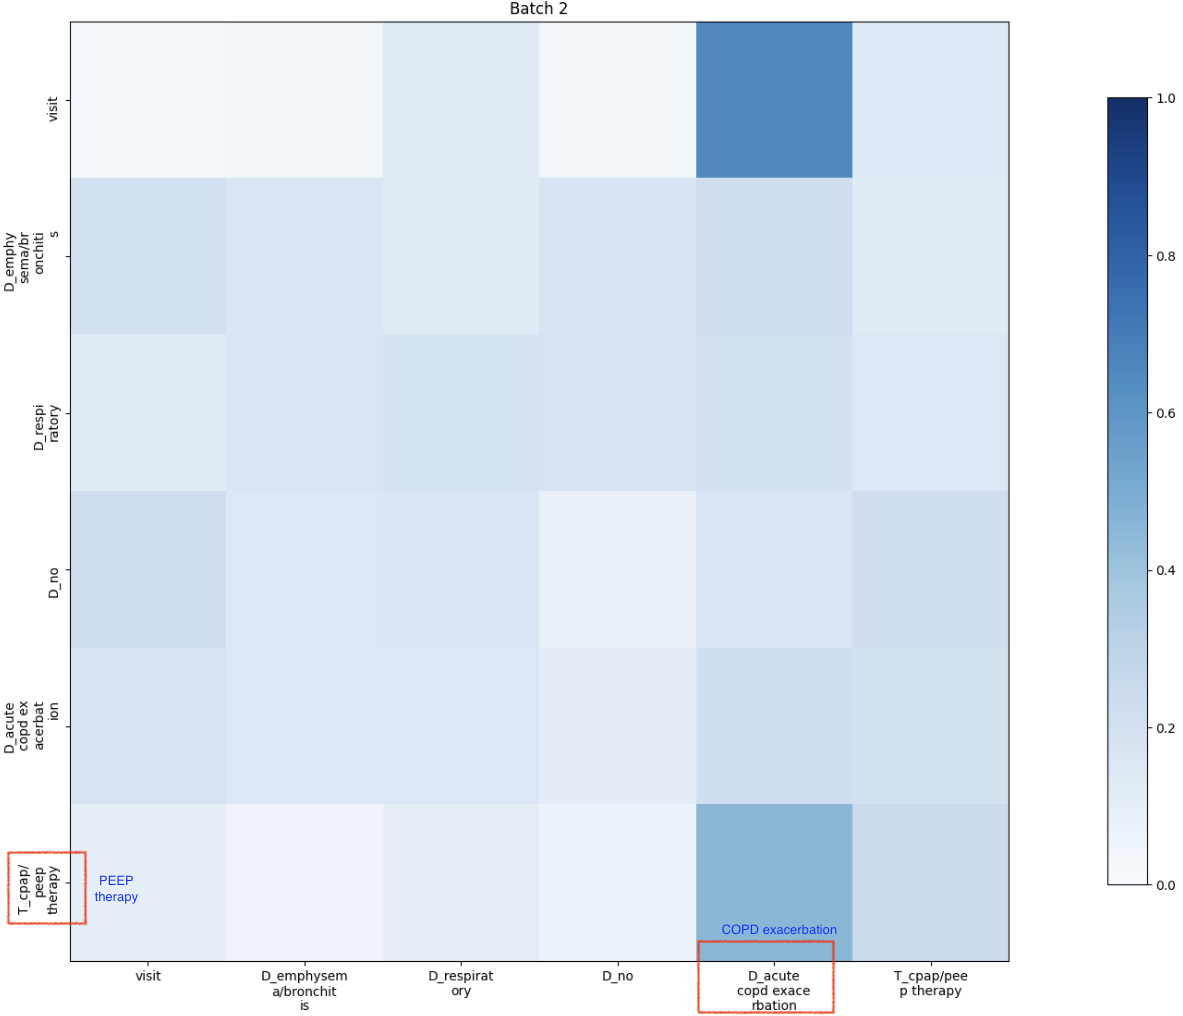
\includegraphics[width=0.5\textwidth]{Attention Map2.png}
    \caption{The heatmap demonstrates that the attention mechanism has learned meaningful relationships between the components. According to the chart,  during this encounter, the primary reason for the visit was COPD exacerbation, and PEEP therapy was found to be the most closely associated treatment for the patient.}
    \label{fig:attention-map2}
\end{figure}

\section{Discussion}
% Implications of the experimental results, whether the original paper was reproducible, and if it wasn’t, what factors made it reproducible
Based on our training results, we evaluate the prediction results of GCT and the effects of different hyperparameters and model configurations. We also conducted some baseline comparisons with the Transformer, GCN, and reduced the number of Transformer stacks to evaluate whether the GCT model is aligned with the stated claims. In general, with our training settings, GCT performed consistently better than these baselines, and the visualization results also indicate that the Self-Attention blocks are capable of capturing the structure connections, thus providing a better visit representation for the specified prediction tasks. However, we cannot reproduce the exact prediction performance as stated in the original paper. Some other researchers attempting to replicate the model also faced a similar issue, and one potential issue of this is due to some unsolved bug in the open-sourced eICU pre-processing script
\footnote{https://github.com/Google-Health/records-research/issues/6}
\footnote{https://github.com/Google-Health/records-research/issues/13}.

\subsection{What was easy}
We could take advantage of various online resources, which helped us understand the structure of GCT and its implementation more efficiently. Additionally, we also found a PyTorch version of the model on a public GitHub repository. Therefore, it was relatively easy to get started reproducing the original paper.

\subsection{What was difficult}
During the model experiments, we found that training and testing the model took a minimum of 6 or 7 hours, which made it difficult to change the parameters and observe changes in performance.

Additionally, we encountered some challenges when attempting to integrate GCT into PyHealth. Firstly, we had to modify the training data format to compute the prior probability. This was difficult because the preprocessing pipeline differed from other standard PyHealth models. Secondly, like other PyHealth models, GCT needs to handle the required input parameter, \texttt{mode}. However, the model currently produces a probabilities dimension based on the specified number of labels in the argument values of \texttt{num\_labels}. Lastly, the calculation process of prior information requires the specification of vocabulary sizes to shape the tensor in the same size. Conversely, in PyHealth model modules, data statistics information is not included, and users are not required to know or specify this information as input parameters.

To make the GCT compatible with PyHealth data pipeline frameworks, we have modified the PyHealth library (details refer to \ref{subsec:PyHealthContrib}) and include an additional preprocessing pipeline on top of the eICUDataset parser. We also created a trainer that is similar to the one in PyHealth model and reimplemented the GCT forward function such that it is compatible with our designed pipeline.

% The following list outlines the efforts we have made thus far. These can be accessed in \textit{gct-pyhealth} under the repository\footnote{https://github.com/lycpaul/dl4h-gp30-gct.git}.
% \begin{itemize}
%     \item modified the model's running method by replacing the bash argument parameters with the parameters in the model initialization. 

%     % \item removed unused \texttt{IntermediateLayer}, and \texttt{SelfOutput} classes in GCT model class.

%     % \item now the processing script\footnote{https://github.com/lycpaul/dl4h-gp30-gct/blob/gct-pyhealth/gct-pyhealth/archive/process\_encounters.py}\footnote{https://github.com/lycpaul/dl4h-gp30-gct/blob/gct-pyhealth/gct-pyhealth/archive/process\_eicu\_dataset.py} handles PyHealth data structures such as Event, Visit, and Patient. Also, the script utilizes eICUDataset modules and readmission, mortality prediction tasks in PyHealth.
% \end{itemize}

\subsection{Recommendations for reproducibility}
To fully utilize the available information in the eICU dataset, we recommend dedicating sufficient time to explore it. The proposed model heavily relies on the given data to extract valuable insights. Specifically, the model leverages masks and conditional probability, constructed by processing the eICU data, to provide prior information to the model. This plays a vital role in the model prediction of graph connections with higher accuracy.

\subsection{Descriptive Notebooks}
We have also included descriptive notebooks in the GitHub repository\footnote{https://github.com/lycpaul/dl4h-gp30-gct/tree/main/gct-pytorch/notebooks} to help with understanding the overall code flow. Another set of notebooks provides a step-by-step walkthrough of the data preprocessing, model training, and evaluation process \footnote{https://github.com/lycpaul/dl4h-gp30-gct/tree/main/gct-pyhealth}. They also include visualizations of the model's attention maps.

\subsection{PyHealth Contribution}
\label{subsec:PyHealthContrib}
Three main modifications have been made in the PyHealth library and merged to the “master” branch recently\footnote{https://github.com/sunlabuiuc/PyHealth/pull/148}.
\begin{itemize}
\item Updated \texttt{parse\_diagnosis()} for parsing the additional diagnosisString columns required in this paper.

\item Added \texttt{parse\_admissiondx()} to parse admissionDX table in eICUDataset of the PyHealth Datasets modules.

\item New prediction tasks are also included to parse the required feature key sets, namely \texttt{mortality\_prediction\_eicu\_fn2()} and \texttt{readmission\_prediction\_eicu\_fn2()}.
\end{itemize}

\newpage
\bibliographystyle{acl_natbib}
\bibliography{acl2021}

\end{document}